% Drawing 138/03-6 -- folder 138, batch 03, archive page 52 (PDF page 53).
% Transcription: un diagramme de revêtements, trop surchargé pour être mis en \texttt{tikz-cd} sans choisir entre des flèches biffées. On y lit : $X_2(p,q,r) \to X_2$ (étiquette $\mu_p \times \mu_q \times \mu_r$) ; $\widetilde{X}_2(p,q,r) \to \widetilde{X}_2$ (étiquette biffée, puis $\mu_{2p} \times \mu_{2q} \times \mu_{2r} \times \pi_n$ ?) ; $X_2(2,2,2) = \widetilde{X}_2 \to X_2$ (étiquette $\mu_2^{3}$) et $\widetilde{X}_2 \to X_4$ (étiquette $\mu_2$) ; $\widetilde{X}_2(n) \to \widetilde{X}_2$ (étiquette $\pi_n$) et $\widetilde{X}_2(n) \to X_{4n}$ (étiquette $\mu_{2n}$ ?) ; $X_{4n} \to X_4$ (étiquette $\pi_4$) ; $X_4 \to X_2$ (étiquette $\pi_2$), $X_4 \to X_1$ (étiquette $\pi_4$) ; $X_2 \to X_1$ (étiquette $\pi_2$) ; une longue flèche de la droite vers $X_2$ sous une étiquette très biffée ($\mu_2^{3}$ ?), et une flèche courbe de $X_1$ vers la droite, étiquetée $\pi_{2n}$ ; un grand arc part du bas et remonte vers $\widetilde{X}_2(p,q,r)$.
% Kind: diagram of coverings (overloaded). Method 2 (schematic redraw from the facsimile). Status: partial.
% Notes: The overloaded diagram of coverings, redrawn as nodes and arrows as far as they can be followed: X_2(p,q,r) -> X_2; X~_2(p,q,r) = X_2(2p,2q,2r) -> X_2(2,2,2) = X~_2; X~_2(p,q,r) (top, written « X~(p,q,r;n) ») -> X~_2 under mu_2p x mu_2q x mu_2r x pi_n ?; X~_2(n) -> X~_2 (pi_n) and -> X_4n (mu_2n ?); X_4n -> X_4 (pi_4); X~_2 -> X_4 (mu_2); X_4 -> X_2 (pi_2) and -> X_1 (pi_4); X_2 -> X_1 (pi_2); a long arrow from the right to X_2 under a heavily struck label; the curved arrow pi_2n along the bottom and the large arc rising to the top node. Which end of the two long curves carries the head is a reading; struck labels are grey. The formulas at the top and right of the page are text of the transcription.
% Coordinates: 1 unit = 1 mm = 1/100 of the crop width (bbox in page fractions: [0.08, 0.15, 0.76, 0.51]).
% Redrawn by Claude (claude-opus-5-5), issue #73, 2026-11-07; not checked by a human; not compiled (no TeX in the session).
% Rights: reproduces part of the work -- behind RENDER_TRANSCRIPTS, never published by itself.
\documentclass[tikz,border=3pt]{standalone}
\usepackage{amsmath,amssymb}
\usetikzlibrary{patterns,arrows.meta}
\tikzset{pencil/.style={black!45}, struck/.style={black!35}, mark/.style={circle,draw,inner sep=1.3pt}, pt/.style={circle,fill,inner sep=0.9pt}, opt/.style={circle,draw,fill=white,inner sep=1.1pt}}
\begin{document}
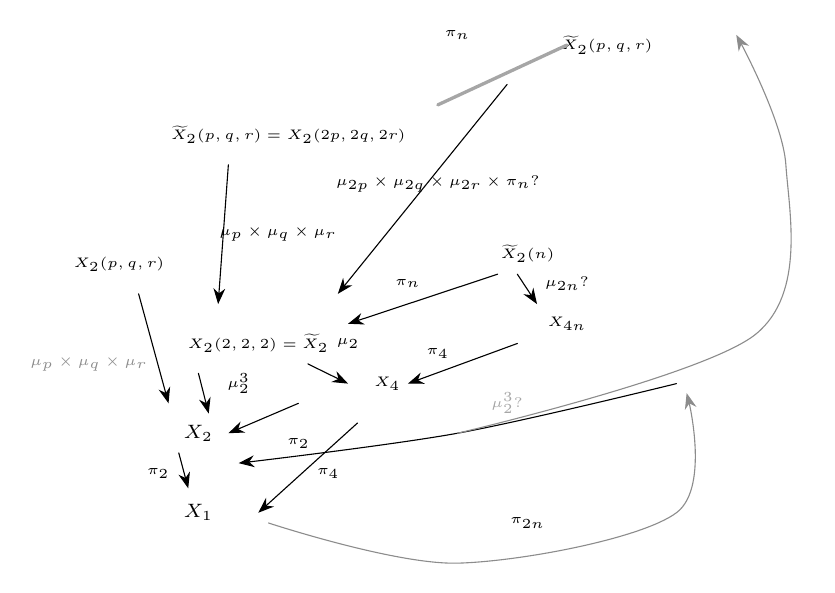
\begin{tikzpicture}[x=1mm,y=1mm,line cap=round,line join=round,font=\scriptsize]
\node[inner sep=1pt] at (69.6,-10.4) {\tiny $\widetilde X_2(p,q,r)$};
\node[inner sep=1pt] at (50.6,-9.1) {\tiny $\pi_n$};
\node[inner sep=1pt] at (29.1,-21.8) {\tiny $\widetilde X_2(p,q,r)=X_2(2p,2q,2r)$};
\node[inner sep=1pt] at (7.6,-38.2) {\tiny $X_2(p,q,r)$};
\node[inner sep=1pt] at (59.5,-36.9) {\tiny $\widetilde X_2(n)$};
\node[inner sep=1pt] at (25.3,-48.3) {\tiny $X_2(2,2,2)=\widetilde X_2$};
\node[inner sep=1pt] at (64.5,-45.8) {\tiny $X_{4n}$};
\node[inner sep=1pt] at (41.7,-53.4) {\tiny $X_4$};
\node[inner sep=1pt] at (17.7,-59.7) {\scriptsize $X_2$};
\node[inner sep=1pt] at (17.7,-69.8) {\scriptsize $X_1$};
\draw[very thick,struck] (64.5,-10.4) -- (48.1,-18);
\draw[-{Stealth[length=2mm]}] (56.9,-15.4) -- (35.4,-42);
\node[inner sep=1pt] at (48.1,-28.1) {\tiny $\mu_{2p}\times\mu_{2q}\times\mu_{2r}\times\pi_n$?};
\draw[-{Stealth[length=2mm]}] (21.5,-25.6) -- (20.2,-43.3);
\node[inner sep=1pt] at (27.8,-34.4) {\tiny $\mu_p\times\mu_q\times\mu_r$};
\draw[-{Stealth[length=2mm]}] (10.1,-42) -- (13.9,-55.9);
\node[inner sep=1pt,pencil] at (3.8,-50.9) {\tiny $\mu_p\times\mu_q\times\mu_r$};
\draw[-{Stealth[length=2mm]}] (55.7,-39.5) -- (36.7,-45.8);
\node[inner sep=1pt] at (44.3,-40.7) {\tiny $\pi_n$};
\draw[-{Stealth[length=2mm]}] (58.2,-39.5) -- (60.7,-43.3);
\node[inner sep=1pt] at (64.5,-40.7) {\tiny $\mu_{2n}$?};
\draw[-{Stealth[length=2mm]}] (58.2,-48.3) -- (44.3,-53.4);
\node[inner sep=1pt] at (48.1,-49.6) {\tiny $\pi_4$};
\draw[-{Stealth[length=2mm]}] (31.6,-50.9) -- (36.7,-53.4);
\node[inner sep=1pt] at (36.7,-48.3) {\tiny $\mu_2$};
\draw[-{Stealth[length=2mm]}] (17.7,-52.1) -- (19,-57.2);
\node[inner sep=1pt] at (22.8,-53.4) {\tiny $\mu_2^3$};
\draw[-{Stealth[length=2mm]}] (30.4,-55.9) -- (21.5,-59.7);
\node[inner sep=1pt] at (30.4,-61) {\tiny $\pi_2$};
\draw[-{Stealth[length=2mm]}] (37.9,-58.4) -- (25.3,-69.8);
\node[inner sep=1pt] at (34.2,-64.8) {\tiny $\pi_4$};
\draw[-{Stealth[length=2mm]}] (15.2,-62.2) -- (16.4,-66.7);
\node[inner sep=1pt] at (12.6,-64.8) {\tiny $\pi_2$};
\draw[-{Stealth[length=2mm]}] plot[smooth, tension=0.55] coordinates {(78.4,-53.4) (50.6,-59.7) (22.8,-63.5)};
\node[inner sep=1pt,struck] at (56.9,-55.9) {\tiny $\mu_2^3$?};
\draw[-{Stealth[length=2mm]},pencil] plot[smooth, tension=0.55] coordinates {(26.6,-71.1) (50.6,-76.2) (78.4,-69.8) (79.7,-54.6)};
\node[inner sep=1pt] at (59.5,-71.1) {\tiny $\pi_{2n}$};
\draw[-{Stealth[length=2mm]},pencil] plot[smooth, tension=0.55] coordinates {(50.6,-59.7) (88.5,-47.1) (92.3,-25.6) (86,-9.1)};
\end{tikzpicture}
\end{document}
